% Native vector schematic: radial order only, not an assertion of locality.
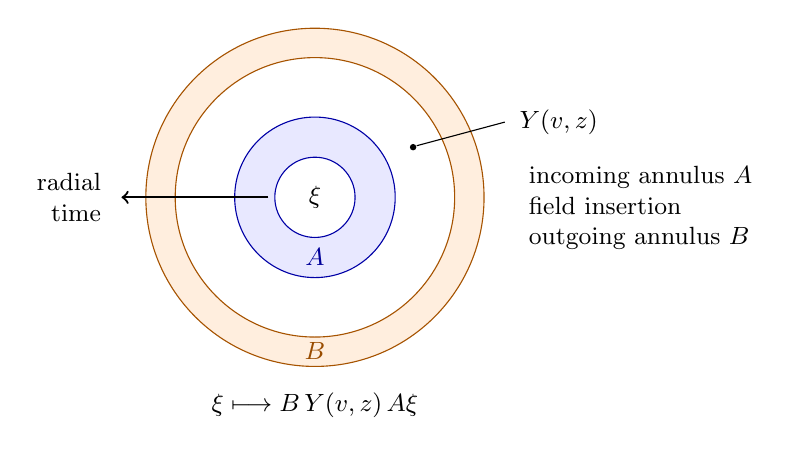
\begin{tikzpicture}[scale=0.91, font=\small]
  \fill[blue!9,even odd rule] (0,0) circle (1.12) (0,0) circle (0.56);
  \fill[orange!13,even odd rule] (0,0) circle (2.36) (0,0) circle (1.95);
  \draw[blue!65!black] (0,0) circle (0.56);
  \draw[blue!65!black] (0,0) circle (1.12);
  \draw[orange!65!black] (0,0) circle (1.95);
  \draw[orange!65!black] (0,0) circle (2.36);
  \node at (0,0) {$\xi$};
  \node[blue!60!black] at (0,-0.83) {$A$};
  \node[orange!60!black] at (0,-2.15) {$B$};
  \fill (1.37,0.70) circle (0.045);
  \draw (1.42,0.72) -- (2.65,1.05);
  \node[anchor=west] at (2.72,1.05) {$Y(v,z)$};
  \draw[->,thick] (-0.65,0) -- (-2.70,0);
  \node[anchor=east,align=right] at (-2.85,0)
       {radial\\time};
  \node[anchor=west,align=left] at (2.85,-0.15)
       {incoming annulus $A$\\field insertion\\outgoing annulus $B$};
  \node at (0,-2.9) {$\displaystyle \xi\longmapsto B\,Y(v,z)\,A\xi$};
\end{tikzpicture}
